\section{Interface - Key Management}


\begin{frame}

\frametitle{Princip}

\underline{Old cryptographic interface (Crypto Wrap)}:
\begin{itemize}
	\item Do not use memory to save several times the same key
\end{itemize}

\vspace{0.25cm}

\underline{New cryptographic interface (GCI)}:

\begin{itemize}
  \item Use of key management to save keys and become an identifiant (ID) of
  where they are saved
  \item Key could be get by passing the ID
  \item Release the key saved to free memory
\end{itemize}

\end{frame}



\begin{frame}

\frametitle{Example of use:}


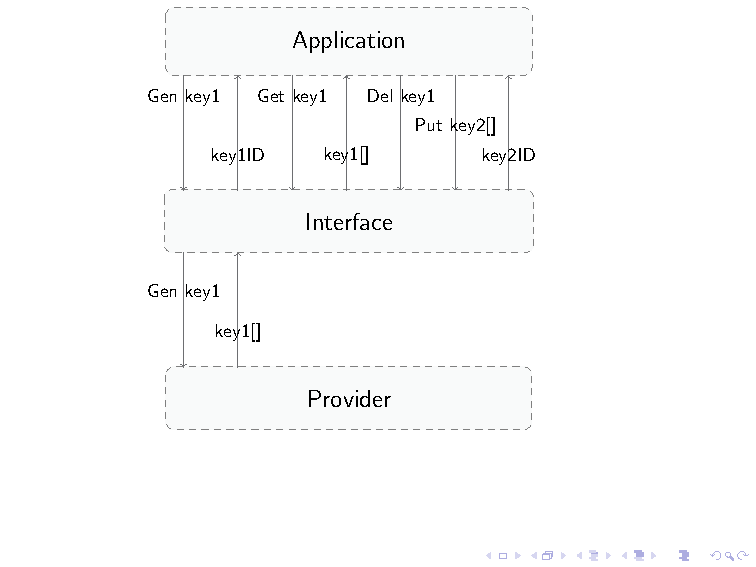
\includegraphics[trim=0.5cm 1cm 14cm 0cm, height=8cm]{figures/key_manag.pdf}


\end{frame}
